\documentclass{report}
\usepackage{graphicx} % Required for inserting images
\usepackage[italian]{babel}
\usepackage{tikz}
\usepackage{hyperref}
\usepackage{amsmath}
\usepackage{xcolor}
\usepackage{float}

\definecolor{darkgreen}{rgb}{0.0, 0.5, 0.0}


\title{Sistemi Biometrici basati sul Volto}
\date{Parte VI}

\begin{document}

\maketitle

\tableofcontents
\newpage

\chapter{Introduzione}

I sistemi biometrici basati sul volto vengono impiegati sia per la \textbf{verifica} dell'identità, che 
per l'\textbf{identificazione}; si possono suddividere in:
\begin{itemize}
    \item 2D
    \begin{itemize}
        \item immagine fissa/video/tante immagini fisse
        \item colori/toni di grigio
    \end{itemize}
    \item 3D
    \begin{itemize}
        \item scansione laser
        \item illuminazione controllata
    \end{itemize}
\end{itemize}

\section{\textcolor{darkgreen}{Vantaggi}}
\begin{itemize}
    \item Ottimo compromesso tra accettabilità dell'utente e prestazioni di accuratezza 
    \item Dispositivi di input adatti a molte condizioni operative 
    \item Risultati direttamente verificabili da un operatore umano 
    \item Permette l'acquisizione non consenziente (video-sorveglianza)
\end{itemize}

\section{\textcolor{red}{Svantaggi}}
\begin{itemize}
    \item Soffrono di elevata variabilità intraclasse 
    \begin{itemize}
        \item posa 
        \item illuminazione
        \item variazioni dell'aspetto dell'individuo (dimagrimento, invecchiamento, \dots)
        \item occlusioni (capelli, occhiali, \dots)
    \end{itemize}
    \item Possibile ingannare i sensori non dotati di sistemi anti-spoofing
    \item Solo di recente le accuratezze sono diventate interessanti per sistemi di larga scala 
\end{itemize}

\section{Non solo identificazione/verifica}
Molti degli algoritmi servono anche per:
\begin{itemize}
    \item riconoscimento delle espressioni facciali 
    \item riconoscimento del movimento delle labbra 
    \item applicazioni di computer grafica 
    \item creazioni di protesi 
\end{itemize}

\section{Principali fasi}
La catena di enroll o verifica/identificazione consiste solitamente nei seguenti passi:
\begin{enumerate}
    \item \textbf{Face Detection} (trovare i volti nelll'immagine)
    \item \textbf{Face Segmentation} (separare il volto dallo sfondo)
    \item \textbf{Face Tracking} (se in un video, deve essere inseguito)
    \item \textbf{Face Normalization} (crop e normalizzazione dell'immagine)
    \item \textbf{Feature Extraction}
    \item \textbf{Matching}
\end{enumerate}

\noindent Le tecniche di deeplearning hanno permesso importanti passi in avanti, specialmente
nelle fasi di \textit{detection}, \textit{segmentation}, \textit{feature extraction} e \textit{matching}.

\section{Intraclasse e interclasse}
\subsection{Variabilità intraclasse}
Moltissimi fattori possono contribuire negativamente sull'accuratezza dei sistemi basati sul 
volto, aumentando la variabilità intraclasse, tra cui:
\begin{itemize}
    \item illuminazione 
    \item espressioni del volto 
    \item posa
    \item occlusioni 
    \item sensori 
    \item invecchiamento 
\end{itemize}

\noindent Le differenze di illuminazione e posa sono quelle 
con i maggiori impatti sulle performance.

\subsection{Similitudine interclasse}
Similitudine tra volti, ad esempio nel caso di:
\begin{itemize}
    \item gemelli 
    \item fratelli, genitori (distanti nel tempo)
    \item sosia
\end{itemize}

\subsubsection{Contributo della genetica}
\textbf{Solo una porzione tra 0,1\% e 0,5\% è diversa per ogni individuo}, tutto 
il resto è uguale per tutti gli esseri umani.

\noindent Tra padre e figlio \textbf{la differenza viene dimezzata}.

\section{Standard}

\subsection{Standard per l'acquisizione}
L'ICAO (\textit{Organizzazione Internazionale per l'Aviazione Civile}) e moltissimi 
governi hanno iniziato a dettare regole stringenti per l'acquisizione del tratto 
biometrico (per passaporti, \dots).

\noindent L'obiettivo è quello di arrivare ad impiegare sistemi sempre più accurati.

\subsection{Standard per il template}
Tutti i venditori di sistemi biometrici hanno il loro algoritmo per la creazione
del template, spesso \textbf{segreto} e/o \textbf{sotto brevetto}.

$\rightarrow$ \textbf{non è possibile interoperabilità} tra i sistemi (caso opposto 
a quello delle impronte digitali nel caso delle minuzie) a meno che vengano
condivise le foto originali e non i template.

\noindent L'ICAO impone anche degli standard sul formato delle foto per i 
\textit{Machine Readable Travel Document (MRTD, ad esempio ePassport)}, tra cui:
\begin{itemize}
    \item risoluzione dell'immagine 
    \item dimensione approssimativa dell'immagine
\end{itemize}

\section{Trend di ricerca}
\begin{itemize}
    \item Affrontare ambienti \textit{unconstrained}
    \begin{itemize}
        \item \textit{outdoor facial images}
        \item \textit{non-frontal facial images}
    \end{itemize}
    \item Affrontare grandi numeri 
    \begin{itemize}
        \item migliorare i tassi di falsi positivi 
        \item \dots
    \end{itemize}
    \item Miglioramenti teorici 
    \begin{itemize}
        \item Il deeplearning continua ad essere uno dei più promettenti
    \end{itemize}
\end{itemize}



\chapter{Algoritmi di prefiltraggio ed estrazione di caratteristica}

\section{Face Detection}
È il primo passo della catena, ha il compito di rintracciare 
il volto/i senza nessun prerequisito particolare; possono cambiare:
\begin{itemize}
    \item condizioni di luce
    \begin{itemize}
        \item intensità
        \item direzione 
        \item banda spettrale 
    \end{itemize}
    \item i volti 
    \begin{itemize}
        \item colore 
        \item posizione 
        \item scala 
        \item posa 
        \item espressione 
    \end{itemize}
\end{itemize}

\begin{figure}[ht]
    \centering
    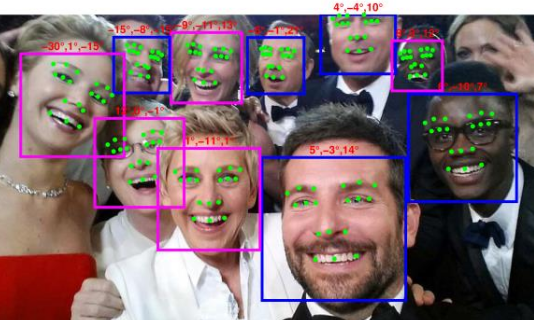
\includegraphics[width=0.7\linewidth]{images/face-detection.png}
\end{figure}

\noindent Molti approcci sono basati su modelli molto semplici del volto, in termini 
\begin{itemize}
    \item geometrici
    \item di texture
\end{itemize}

\noindent Questi modelli permettono di trovare nelle immagini le regioni dove 
\textbf{\textit{fittano} meglio il modello} e quindi dove \textbf{è maggiore 
la probabilità che ci sia un volto}.

\subsection{Color based}
Nel caso delle immagini a colori uno degli schemi più diffusi
è il seguente:
\begin{enumerate}
    \item lighting compensation 
    \item skin tone detection 
    \item localization of facial features (occhi, bocca, contorno del viso)
    \item aggregazione dei risultati
\end{enumerate}

\begin{figure}[ht]
    \centering
    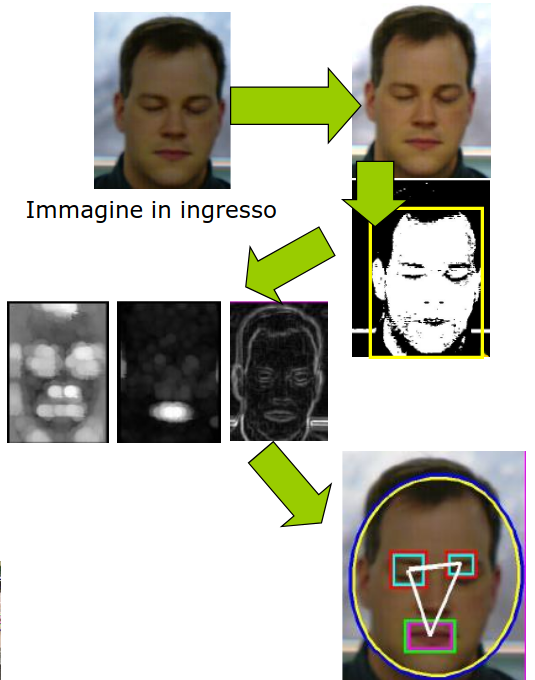
\includegraphics[width=0.58\linewidth]{images/fd-color-based.png}
\end{figure}

\noindent La skin tone detection viene effettuata controllando 
quali bit dell'immagine appartengono ad una determinata
regione dello spazio colore che evidenzia meglio le differenze.

\begin{figure}[ht]
    \centering
    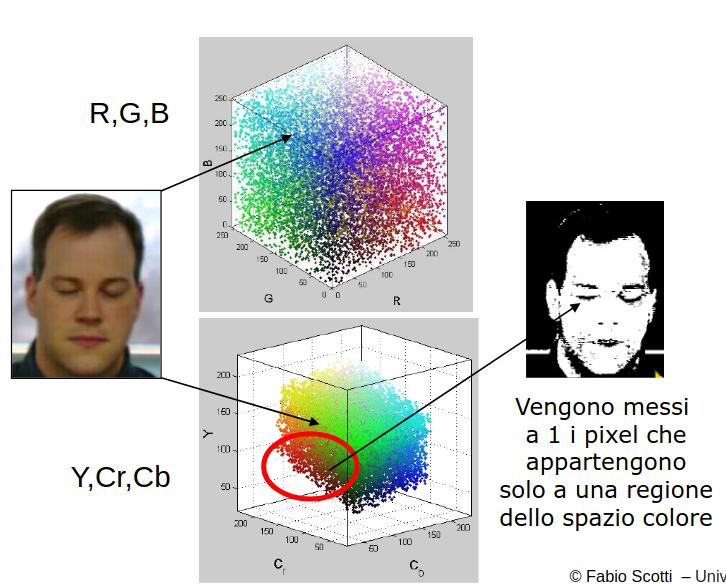
\includegraphics[width=0.7\linewidth]{images/fd-color-based2.png}
\end{figure}

\noindent La rilevazione della posizione degli occhi e della 
bocca viene effettuata sottraendo immagini espresse in appositi 
spazi colore che ne possano mettere in evidenza le \textbf{caratteristiche 
cromatiche peculiari}.

\subsection{Haar feature}
Il metodo delle feature basate su funzioni di Haar consiste 
nel cercare nelle immagini delle regioni che presentano 
particolari vaori delle \textit{trasformate di Haar};
solitamente i \textbf{i volti sono caratterizzati da particolari 
valori} e quindi si possono trovare tramite dei classificatori.

\section{Face tracking}
Quando si ha a che fare con un video si deve svolgere il face tracking;
non è esattamente come fare del face detection in ogni frame, dato che:
\begin{itemize}
    \item si hanno maggiori informazioni da un filmato (i volti non possono 
    essersi spostati di molto da un frame all'altro)
    \item avendo due frame è possibile effettuare una previsione sullo spostamento 
    del volto o sulle sue deformazioni
\end{itemize}

\chapter{Estrazione di caratteristica e matching}

\section{Rappresentazione dei volti}
Ogni immagine $p * q$ pixel viene rappresentata come un punto 
nello spazio $R^n$, con $n = p * q$

\noindent Si crea così lo \textbf{spazio delle facce}.

\begin{figure}[ht]
    \centering
    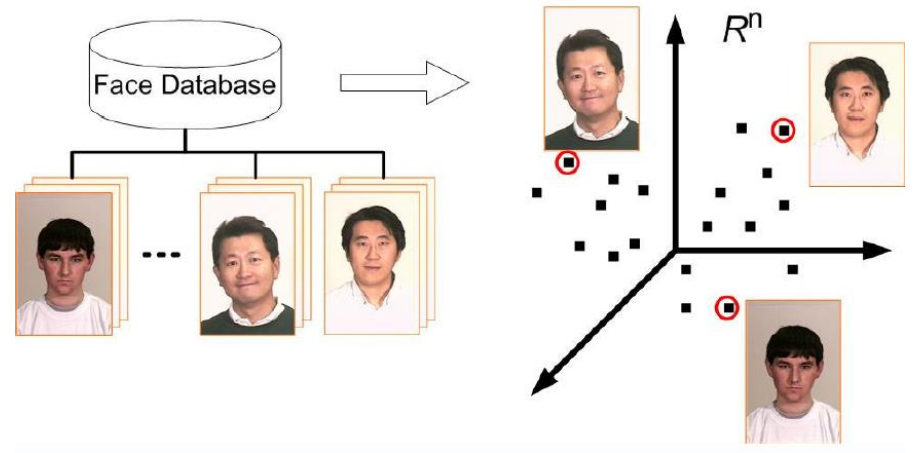
\includegraphics[width=0.8\linewidth]{images/spazio-facce.png}
\end{figure}

$\rightarrow$ problema: è uno spazio ad altissima dimensionalità

\subsection{Analisi lineare di un sottospazio delle facce}
Lo spazio delle facce costruito con le immagini raw ha una dimensionalità
troppo elevata; le facce possono risiedere in uno sottospazio limitato 

$\rightarrow$ il modo di stabilire il sottospazio crea il metodo di analisi

\noindent Bisogna trovare una \textbf{trasormazione lineare che mappa il vettore
di immagini X in un sottospazio} di dimensione $l$ molto più 
limitata $(l << n)$; il match avverrà sulle feature delle immagini ottenute.

\section{Analisi lineare di un sottospazio mediante PCA}

La tecnica PCA (\textit{Principal Component Analysis}) cerca una rotazione 
dello spazio (ancora la dimensionalità non cambia) che \textbf{permette di 
separare meglio le classi}.

\begin{figure}[ht]
    \centering
    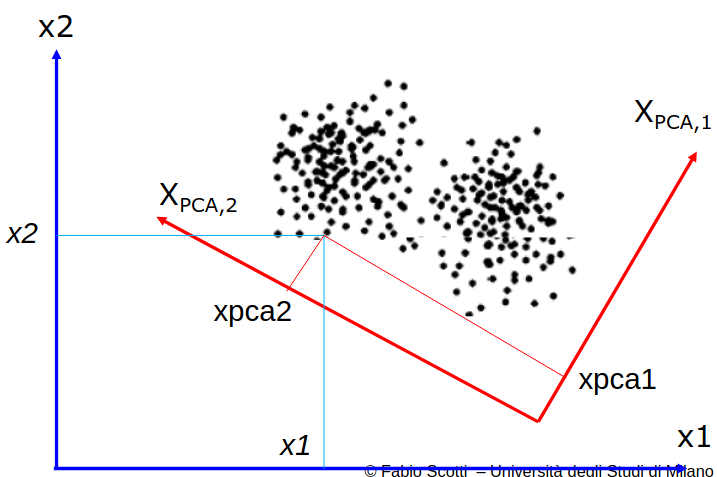
\includegraphics[width=0.7\linewidth]{images/pca.png}
\end{figure}

\noindent È possibile passare da un sistema di coordinate ad un altro tramite una moltiplicazione
tra matrici.

$\rightarrow$ \textbf{PCA cerca una rototraslazione} che permette di 
mettere la variabilità dei dati tutta nei primi parametri.

\subsection{Vantaggi e Svantaggi}

\begin{itemize}
    \item \textcolor{darkgreen}{\textbf{Vantaggi}}
    \begin{itemize}
        \item compatta la maggior parte della varianza nel minor numero di coefficienti di trasformazione 
        \item riduce lo spazio dei dati in ingresso
        \item minimizza errore medio tra i dati ricostruiti e quelli originali 
        \item minimizza entropia totale dei dati costruiti 
    \end{itemize}
    \item \textcolor{red}{\textbf{Svantaggi}}
    \begin{itemize}
        \item non ci sono algoritmi veloci per la sua implementazione 
        \item è costoso in termini di risorse computazionali
    \end{itemize}
\end{itemize}

\newpage
\subsection{Creazione DB e distanze tra utenti diversi}
\begin{figure}[H]
    \centering
    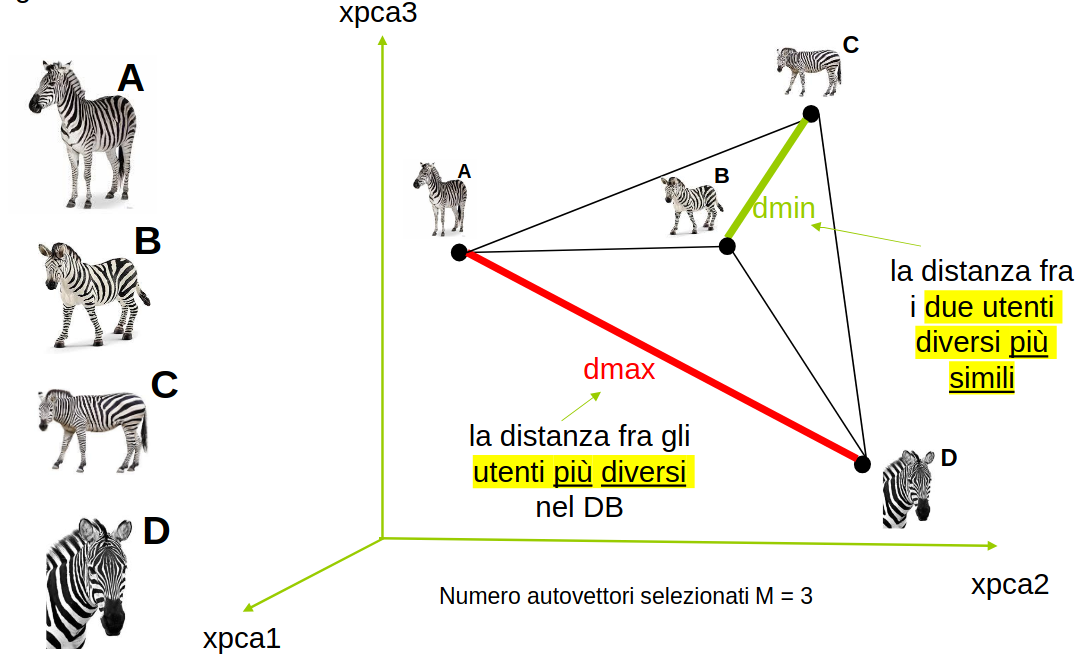
\includegraphics[width=1\linewidth]{images/distance1.png}
\end{figure}

\subsection{Arrivo di una faccia nuova - Spazio PCA}
\begin{figure}[H]
    \centering
    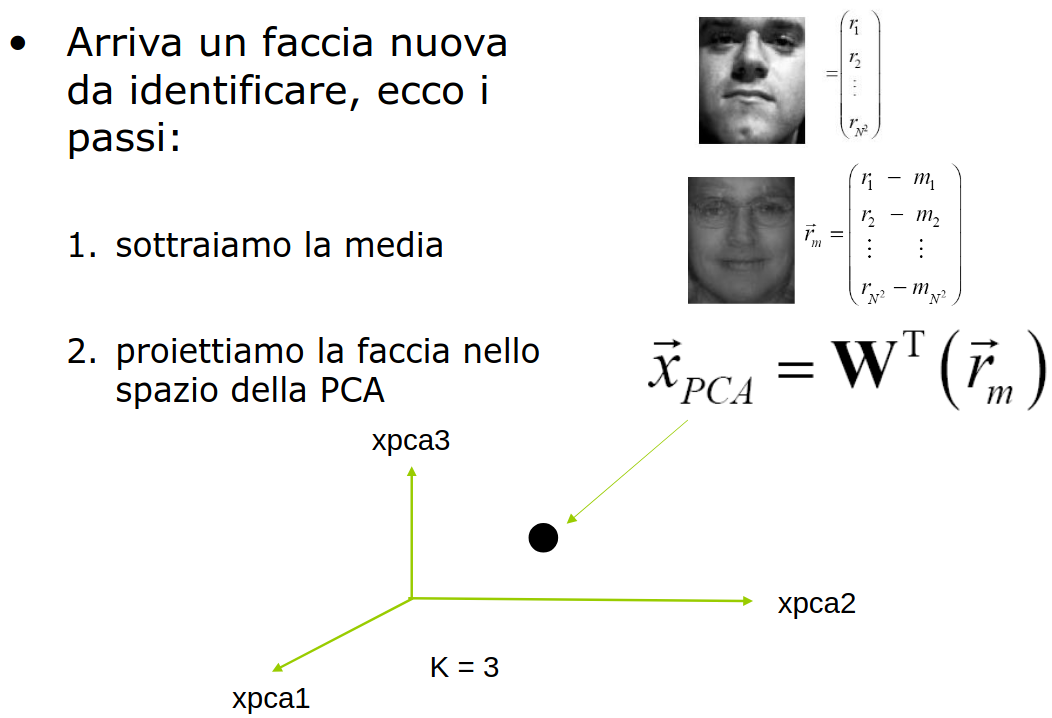
\includegraphics[width=1\linewidth]{images/distance2.png}
\end{figure}

\begin{figure}[H]
    \centering
    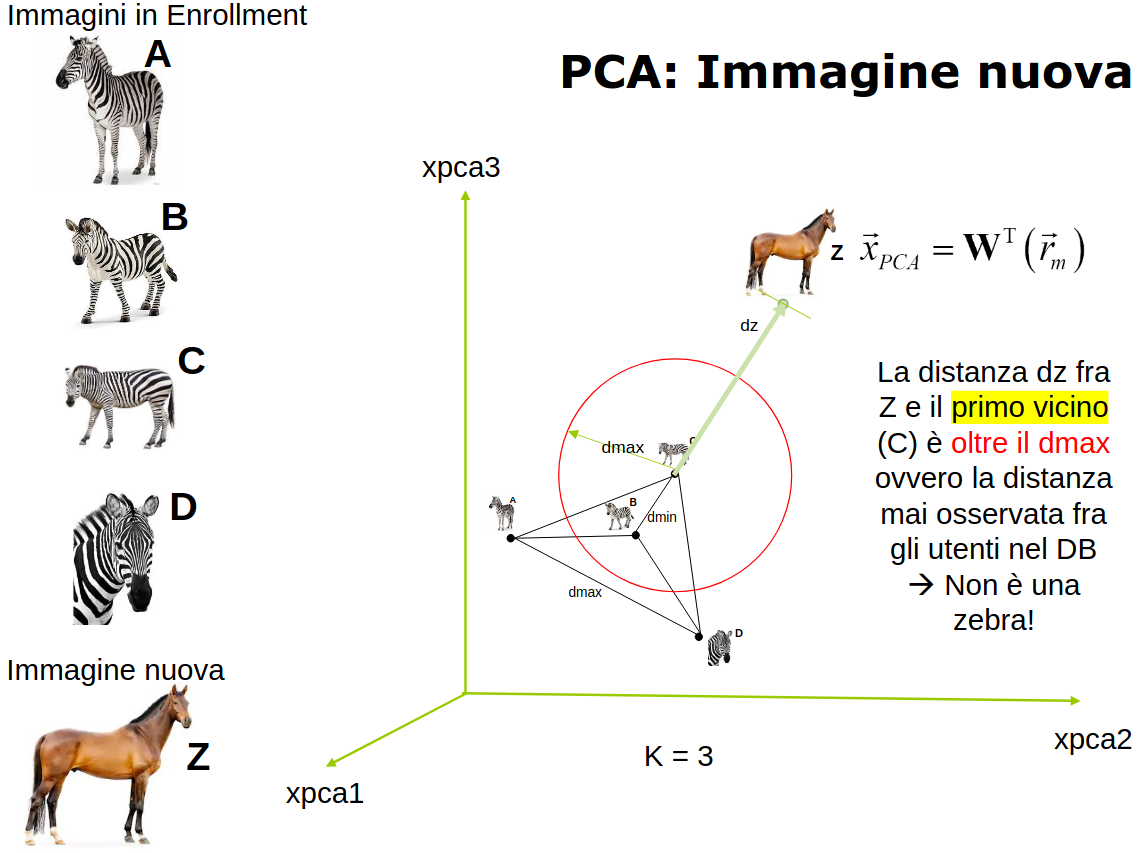
\includegraphics[width=1\linewidth]{images/imm-new.png}
\end{figure}

\begin{figure}[H]
    \centering
    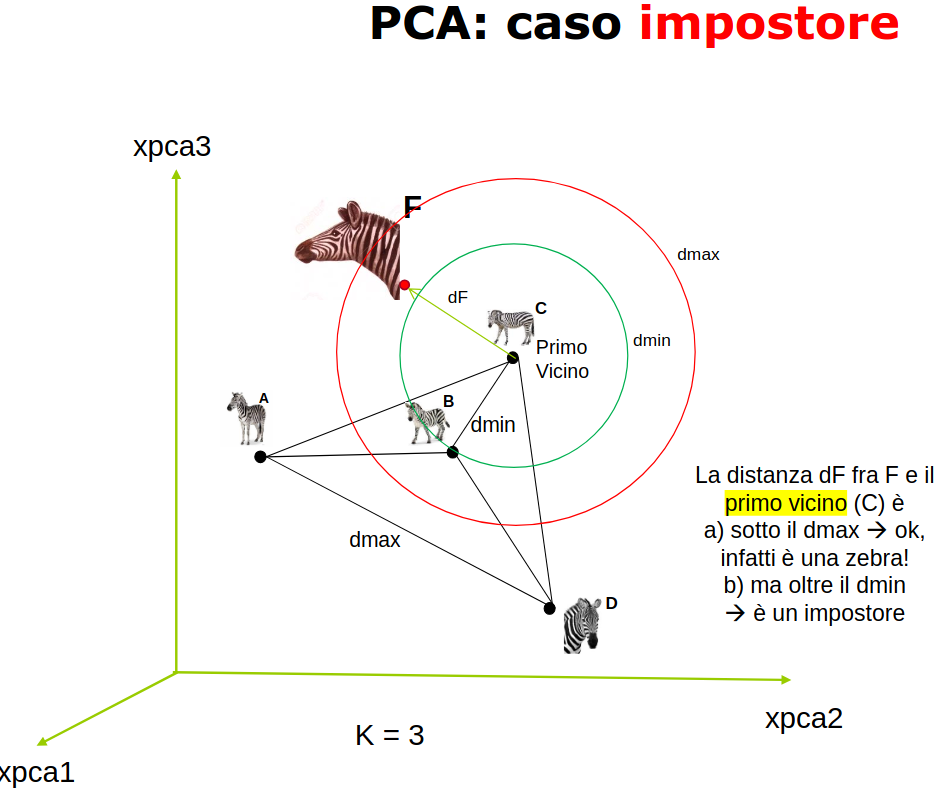
\includegraphics[width=0.9\linewidth]{images/impostore.png}
\end{figure}

\begin{figure}[H]
    \centering
    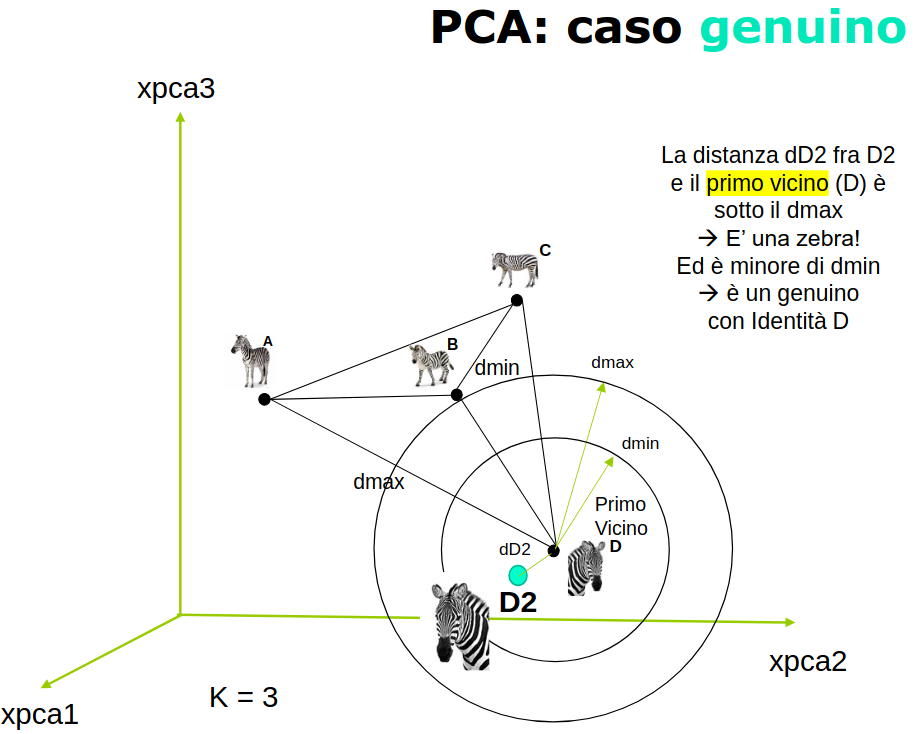
\includegraphics[width=0.9\linewidth]{images/imm-genuino.png}
\end{figure}

\subsection{Spazio delle facce}
All'arrivo di una nuova faccia, la possiamo classificare
usando anche lo spazio delle facce:
\begin{enumerate}
    \item Ricostruiamo la faccia usando le autofacce
    \item Calcoliamo la distanza della faccia ricostruita da quella iniziale
\end{enumerate}

\noindent L'errore indica quanto \textbf{l'immagine iniziale era vicina alle immagini con 
cui abbiamo calcolato le autofacce}; quindi quanto probabilmente potrebbe 
essere genuino o un impostore
\begin{itemize}
    \item se ricostruisco bene l'immagine nuova (l'errore è basso) allora probabilmente era 
    un'immagine simile a quelle memorizzate 
    \item se il volto è troppo diverso rispetto a tutti quelli del DB del autofacce (l'errore è alto), allora è un impostore
\end{itemize}

\newpage
\subsection{Significato delle autofacce}
\begin{itemize}
    \item \textbf{Enroll:} dai volti si calcolano le autofacce con la tecnica PCA
    \item \textbf{Verification:} Ogni volto del DB può essere ricostruito esattamente con una 
    combinazione lineare di autofacce; se un nuovo volto viene ricostruito male, allora:
    \begin{itemize}
        \item non è un volto 
        \item è un impostore
    \end{itemize}
\end{itemize}

\subsubsection{Considerazioni sulle autofacce}
Sono una tecnica base, che è stata nel tempo raffinata per far fronte 
agli evidenti svantaggi:
\begin{itemize}
    \item non usano l'informazione di classe (apprendimento non superivisionato), ma 
    lavorano solo sulla distribuzione dei punti nello spazio delle facce
    \item soffrono delle variazioni di 
    \begin{itemize}
        \item illuminazione
        \item posa 
        \item allineamento 
        \item espressioni facciali
    \end{itemize}
\end{itemize}

\newpage
\section{Altri metodi di estrazione delle feature e matching}

\subsection{Metodi di analisi locale}
I metodi di analisi locale lavorano sul riconoscimento, misurazione e 
confronto dei dettagli del volto, come ad esempio:
\begin{itemize}
    \item misure del naso, bocca, distanza tra gli occhi, \dots
    \item valori ritornati da particolari funzioni di trasformazione
\end{itemize}

\begin{figure}[ht]
    \centering
    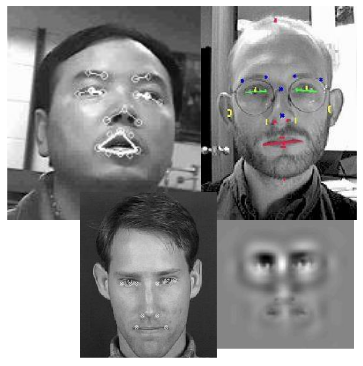
\includegraphics[width=0.4\linewidth]{images/analisi-locale.png}
\end{figure}

\subsection{Metodi \textit{model-based}}
I metodi \textit{model based} estraggono non una feature singola, ma 
adattano un modello sulla faccia trovandone i coefficienti per 
poi confrontarli con quelli delle altre facce.

\begin{figure}[ht]
    \centering
    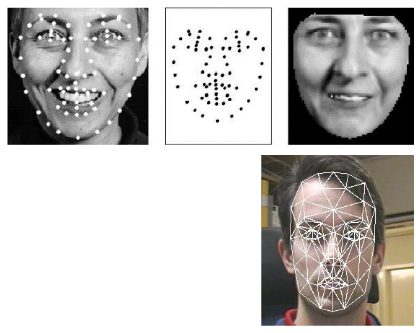
\includegraphics[width=0.5\linewidth]{images/model-based.png}
\end{figure}

\subsubsection{\textit{Graph Matching}}
Nei metodi di \textit{graph matching} il volto è rappresentato 
come una rete di nodi sui punti peculiari del volto; servono 
\textbf{almeno due immagini per trovare il modello del volto} (il grafo).

\noindent La comparazione di due facce viene eseguita misurando 
quanto \textit{sforzo} è necessario fare per adattare un grafo all'altro
\textit{tirando} i nodi, che sono legati ad un modello elastico.

\begin{figure}[ht]
    \centering
    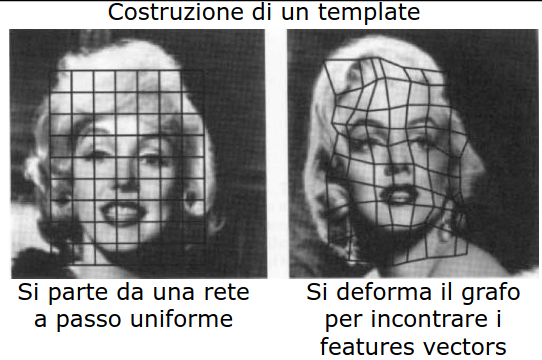
\includegraphics[width=0.8\linewidth]{images/graph.png}
\end{figure}

\chapter{Spoofing e Anti-Spoofing}

\section{Limiti oggettivi e tipi di attacco}
\begin{itemize}
    \item Il volto può essere coperto da peli o indumenti durante 
    le fasi di enrollment o verification
    \begin{itemize}
        \item non accettare acquisizioni se la percentuale coperta supera 
        quella necessaria per garantire l'accuratezza certificata dal sistema
    \end{itemize}
    \item Maschera di pelle artificiale
    \begin{itemize}
        \item tecniche termografiche e spettrometriche a diverse lunghezze d'onda 
        per rilevare la pelle 
    \end{itemize}
    \item Immagine di un volto stampata o proiettata con uno schermo 
    \begin{itemize}
        \item controllo tridimensionalità 
        \item controllo sincronia tratti biomerici indipendenti (esempio 
        variazioni di volto e voce mentre si parla)
    \end{itemize}

\end{itemize}

\section{Attacco Hill Climbing}
\textit{È possibile ricreare un \textbf{sample} da dei \textbf{template}
memorizzati in un sistema?}

$\rightarrow$ \textbf{Sì!} Basta avere accesso al match score

La tecnica \textit{\textbf{Hill Climbing}} prevede di:
\begin{enumerate}
    \item iniziare con un sample casuale 
    \item portare delle piccole modifiche che incrementino il match score 
    \item proseguire finché si riesce ad aumentare il match score
\end{enumerate}

\noindent Per velocizzare il processo si parte da un database locale di 
immagini (accessi trafugati); l'obiettivo è quello di manipolare l'immagine 
di partenza per farla \textit{matchare} con un'immagine target ingannando il sistema.

\begin{figure}[H]
    \centering
    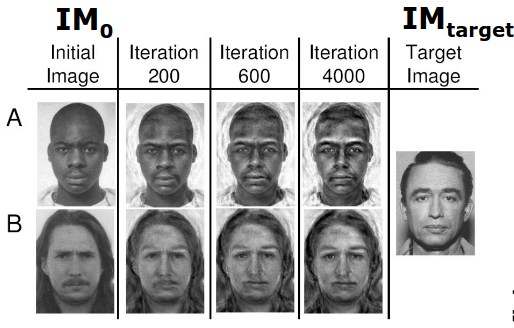
\includegraphics[width=0.8\linewidth]{images/hill-climbing.png}
\end{figure}

\noindent Il problema è che qualunque sia il valore di soglia settato \dots
basta proseguire con le iterazioni e \textit{prima o poi si entra!}

\begin{figure}[H]
    \centering
    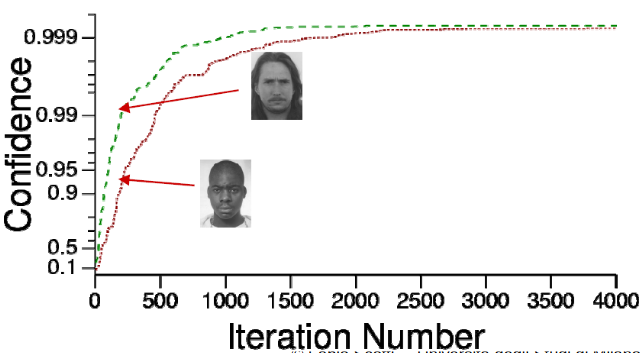
\includegraphics[width=0.8\linewidth]{images/confidence.png}
\end{figure}

\newpage
\section{Metodi di controllo}

\subsection{Controllo della sincronia parlato - movimenti delle labbra}

Il sistema chiede all'utente di pronunciare
di fronte al sensore una frase (casuale) richiesta dal sistema.

\noindent Il sistema misura la variazione dei movimenti delle labbra 
nel tempo controllando se si sta cercando di ingannare il sistema, 
ad esempio con una maschera o con una immagine proiettata.

\subsection{Facial Fingerprinting}
La mappa di vene e capillari al di sotto del volto viene rilevata 
da telecamere ad infrarosso ad alta risoluzione, diventando un nuovo 
tipo di tratto biometrico:
\begin{itemize}
    \item unico 
    \item difficilmente falsificabile 
    \item non intrusivo
    \item accurato
\end{itemize}

\subsection{Controllo istogrammi del colore}
In caso di attacchi con immagini stampate o proiettate, il controllo 
avviene controllando la distribuzione dei colori.

\begin{figure}[ht]
    \centering
    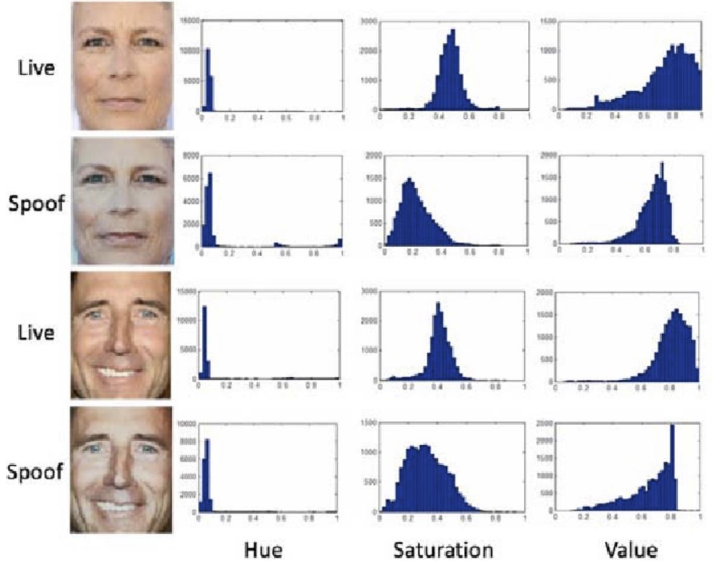
\includegraphics[width=0.8\linewidth]{images/isto.png}
\end{figure}

\subsection{Controllo di pattern}
Quando con una camera si inquadrano delle stampe o display 
avvengono dei particolari pattern; si possono vedere direttamente 
nell'immagine inquadrata o nella \textit{trasformata di Fourier}.

\begin{figure}[ht]
    \centering
    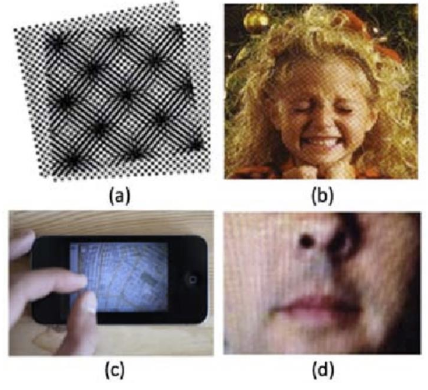
\includegraphics[width=0.6\linewidth]{images/pattern.png}
\end{figure}

\subsection{Infrared Anti-Spoofing}
Le telecamere ad infrarossi offrono un punto di vista diverso 
e più robusto alle condizioni ambientali.

\noindent Inoltre, i display o le stampe diventano non usabili 
con camera IR.

\begin{figure}[ht]
    \centering
    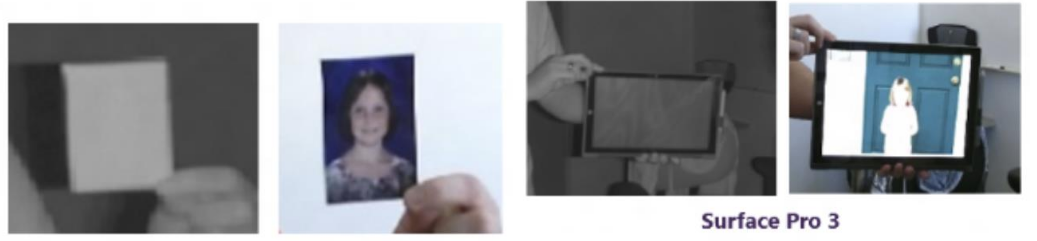
\includegraphics[width=1\linewidth]{images/infrared.png}
\end{figure}

\subsubsection{Analisi 3D}
I dispositivi in grado di scansionare il volume degli oggetti 
possono migliorare le capacità anti-spoofing.

\chapter{Sistemi basati sul volto 3D}

\section{Sensori e caratteristiche}

Attualmente i sistemi biometrici basati sul volto 3D sono in grado di gestire
correttamente acquisizioni frontali con espressione neutra.

\subsection{Acquisizione mediante scanner laser}

\begin{itemize}
    \item Una lama di luce laser scandisce il volto del soggetto durante una ripresa video
    \item Attraverso la geometria spaziale (nota) del sistema si 
    ricostruisce la superificie tramite ogni frame del filmato
\end{itemize}

\begin{figure}[ht]
    \centering
    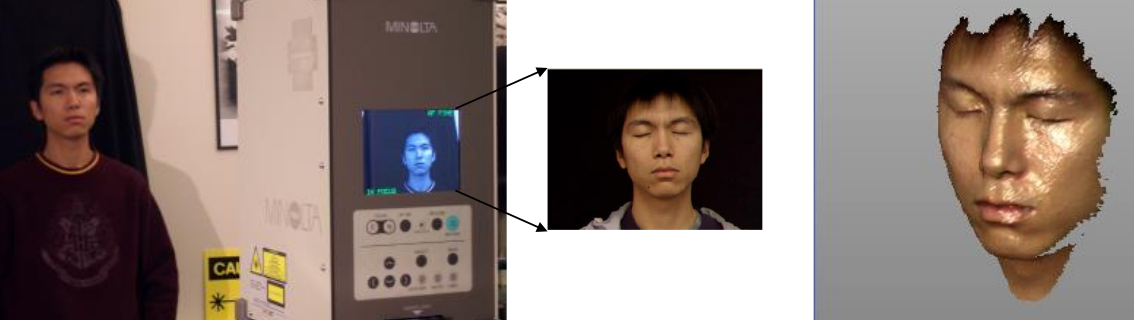
\includegraphics[width=1\linewidth]{images/laser3D.png}
\end{figure}


\subsection{Acquisizione mediante luce strutturata}
\begin{itemize}
    \item Si illumina il volto da riprendere con un proiettore in 
    grado di produrre un fascio di luce strutturata
    \item Si riprende con una o due telecamere
    \item Si proiettano in successione tanti pattern binari, con bande sempre più fini
    \item Il sistema ricostruisce la tridimensionalità usando la deformazione 
    delle bande nell'immagine
\end{itemize}

\begin{figure}[ht]
    \centering
    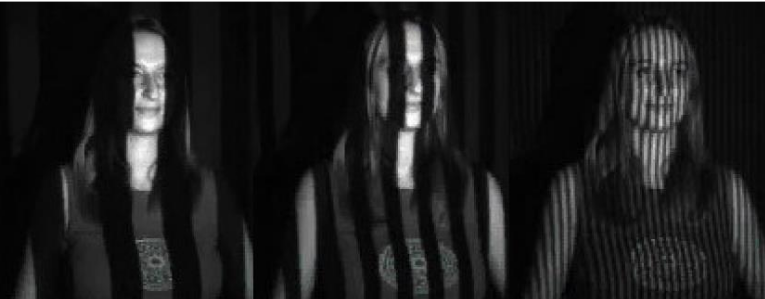
\includegraphics[width=0.67\linewidth]{images/luce-strutturata.png}
\end{figure}

\begin{itemize}
    \item Per aumentare la superficie 3D acquisita si possono usare due tecniche:
    \begin{itemize}
        \item due telecamere 
        \item due acquisizioni indipendenti
    \end{itemize}
    \item Le due superifici 3D che si ottengono poi vanno unite in una sola
\end{itemize}

\subsection{Acquisizione mediante diverse viste}
\begin{itemize}
    \item I sistemi chiamati \textbf{2,5D} riescono a riprodurre la 
    superificie 3D del volto da tante immagini prese da angoli diversi 
    usando una normale telecamera 
    \item Successivamente, si riesce a costruire un vero e proprio modello 3D 
    del volto a partire dalle immagini 2,5D
\end{itemize}

\begin{figure}[ht]
    \centering
    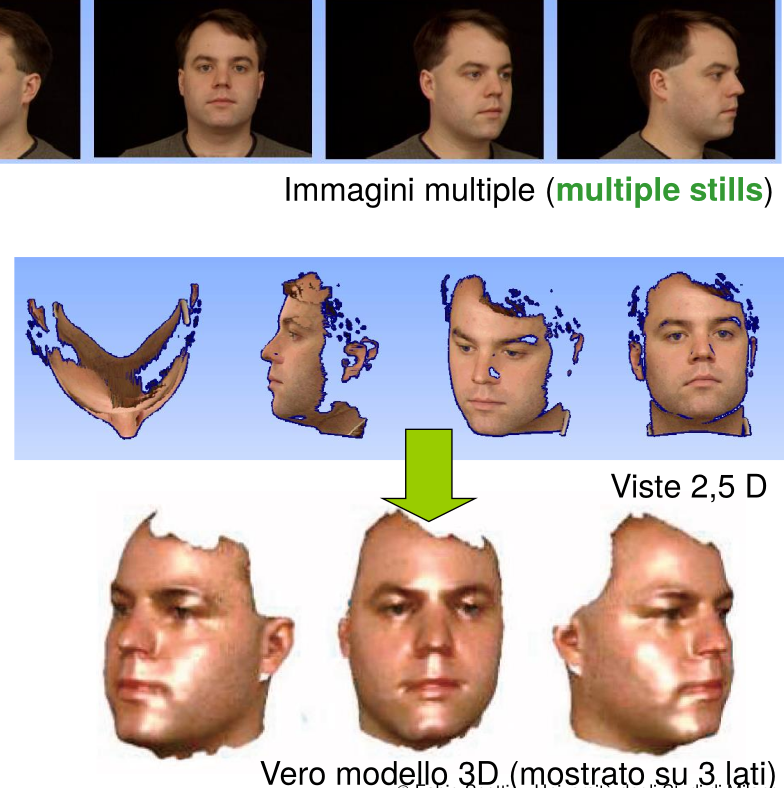
\includegraphics[width=0.6\linewidth]{images/2,5d.png}
\end{figure}

\section{Vantaggi e svantaggi dei sistemi 3D}
\begin{itemize}
    \item \textcolor{darkgreen}{\textbf{Vantaggi}}
    \begin{itemize}
        \item invarianza alla luce ambiente (usando IR)
        \item maggiormente tolleranti rispetto a sfondo, accessori, \dots
        \item invarianti rispetto a piccoli spostamenti angolari del volto 
        \item la precisione di alcuni sistemi permette di distinguire gemelli omozigoti 
        \item prestazioni, sia in termini di tempo che di precisione
    \end{itemize}
    \item \textcolor{red}{\textbf{Svantaggi}}
    \begin{itemize}
        \item costo dei sensori e del sistema 
        \item il soggetto deve essere collaborativo
    \end{itemize}
\end{itemize}

\section{Algoritmi di matching}
Il confronto fra due volti 3D segue i seguenti passi:
\begin{itemize}
    \item Se il volto 3D non è direttamente acquisito dal sensore, tramite acquisizioni 
    multiple si passa ai modelli 3D da confrontare (tipicamente uno dei due volti è già stato memorizzato)
    \item I volti vengono sovrapposti fino a trovare la migliore sovrapposizione 
    \item Si valuta il grado di sovrapposizione con una soglia 
\end{itemize}

\noindent Il match prevede l'individuamento di 3 punti di riferimento per 
facilitare la sovrapposizione delle immagini.

\begin{figure}[ht]
    \centering
    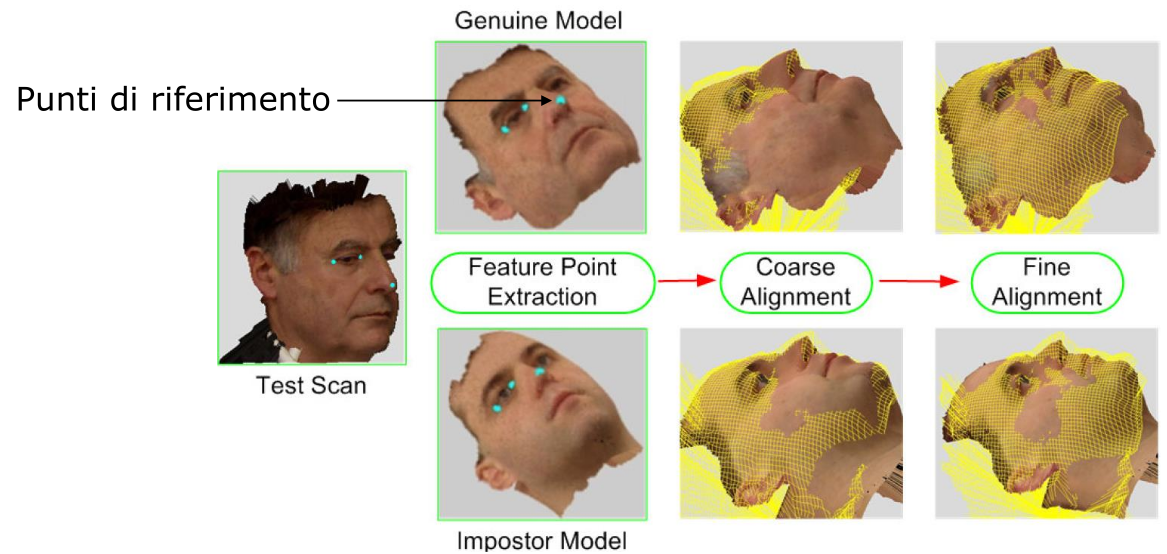
\includegraphics[width=1\linewidth]{images/matching3D.png}
\end{figure}

\section{Prestazioni}
Ci sono notevoli miglioramenti nel \textit{face recognition}, con 
diversi algoritmi che in degli esperimenti sono stati in grado di 
battere degli esseri umani.

\noindent In particolare, ci sono miglioramenti in:
\begin{itemize}
    \item accuratezza
    \item usabilità
    \item numero e tipi di dispositivi in cui poterlo usare 
\end{itemize}

\noindent Queste ragioni sono causa di una crescente diffusione 
preoccupazione sulla privacy degli utenti.



















\end{document}